\documentclass[aspectratio=169,10pt]{beamer}

% ==============================================================================
% Configuración de Tema y Colores (Heredados de presentacion_avances_nandu_emg.tex)
% ==============================================================================
\usetheme{Boadilla}
\usecolortheme{whale}

% Paleta institucional moderna y limpia
\definecolor{DarkBlue}{HTML}{0F172A}
\definecolor{AccentBlue}{HTML}{1E40AF}
\definecolor{SoftBlue}{HTML}{3B82F6}
\definecolor{LightBg}{HTML}{F8FAFC}
\definecolor{CardBg}{HTML}{F1F5F9}
\definecolor{TextDark}{HTML}{0F172A}

\setbeamercolor{palette primary}{bg=DarkBlue,fg=white}
\setbeamercolor{palette secondary}{bg=AccentBlue,fg=white}
\setbeamercolor{palette tertiary}{bg=SoftBlue,fg=white}
\setbeamercolor{structure}{fg=AccentBlue}
\setbeamercolor{frametitle}{bg=DarkBlue,fg=white}
\setbeamercolor{title}{bg=DarkBlue,fg=white}
\setbeamercolor{block title}{bg=AccentBlue,fg=white}
\setbeamercolor{block body}{bg=CardBg,fg=TextDark}

% Opciones tipográficas y paquetes
\usepackage[utf8]{inputenc}
\usepackage[spanish]{babel}
\usepackage{amsmath,amssymb}
\usepackage{graphicx}
\usepackage{booktabs}
\usepackage{microtype}
\usepackage{helvet}
\usepackage{tikz}
\usetikzlibrary{shapes.geometric, arrows.meta, positioning, calc}
\usepackage[most]{tcolorbox}

% Ajuste de márgenes y navegación
\setbeamersize{text margin left=0.6cm, text margin right=0.6cm}
\setbeamertemplate{navigation symbols}{}
\setbeamertemplate{footline}[frame number]

% Configuración del comando de Placeholder de Figuras
\newcommand{\placeholderfigura}[2]{%
    \begin{tcolorbox}[
        colback=CardBg,
        colframe=AccentBlue!75!DarkBlue,
        arc=2mm,
        boxrule=1.1pt,
        halign=center,
        valign=center,
        width=\textwidth,
        height=#1
    ]
        \centering
        \textbf{\color{AccentBlue}\footnotesize [INSERTAR FIGURA: #2]}\\[0.14cm]
        \scriptsize\color{TextDark!70}Colocar imagen en carpeta \texttt{figuras/} y descomentar \texttt{\textbackslash includegraphics}
        % \includegraphics[width=\textwidth,height=#1,keepaspectratio]{figuras/...}
    \end{tcolorbox}%
}

% Título y Metadatos
\title[Acústica y Dinámica Muscular]{De la Acústica del Tracto Vocal a la Dinámica Muscular: Gestos, Lengua y Coarticulación}
\subtitle{Laboratorio de Sistemas Dinámicos - LSD}
\author[S. Prado Rodríguez]{Santiago Prado Rodríguez}
\institute[LSD - UBA]{Laboratorio de Sistemas Dinámicos (LSD) \\ Departamento de Física, FCEyN - Universidad de Buenos Aires}
\date{Noviembre 2026}

\begin{document}

% ------------------------------------------------------------------------------
% Inclusión Modular de Diapositivas
% ------------------------------------------------------------------------------
% ------------------------------------------------------------------------------
% Slide 0: Portada
% ------------------------------------------------------------------------------
\begin{frame}[plain]
    \titlepage
\end{frame}

% ------------------------------------------------------------------------------
% Slide 1: Física del Tracto Vocal: El Modelo de Dos Tubos
% ------------------------------------------------------------------------------
\begin{frame}{Física del Tracto Vocal: El Modelo de Dos Tubos}
    \begin{columns}[c]
        \begin{column}{0.51\textwidth}
            \scriptsize
            \begin{block}{Resonancia y Filtrado Acústico}
                Las vocales se producen mediante el filtrado acústico del tracto vocal sobre el tren de pulsos glóticos, determinando las formantes principales ($F_1$ y $F_2$).
            \end{block}
            \vspace{0.03cm}
            \begin{block}{Aproximación de Dos Tubos Acoplados}
                A primer orden, el tracto se comporta como un \textbf{resonador de Helmholtz doble}: las frecuencias propias dependen del volumen de las cavidades y del área de constricción entre ellas.
            \end{block}
            \vspace{0.03cm}
            \begin{alertblock}{Tres Actuadores Mecánicos Principales}
                \begin{itemize}\setlength{\itemsep}{1pt}\setlength{\parskip}{0pt}
                    \item \textbf{Bajar la mandíbula:} abrir la boca con el digástrico, agranda la cavidad bucal y sube $F_1$.
                    \item \textbf{Estirar los labios adelante:} hacer trompita con el orbicular, alarga el tubo acústico y baja $F_2$.
                    \item \textbf{Mover la lengua:} la posición de la lengua adentro cambia el volumen de cada tubo y fija $F_2$.
                \end{itemize}
            \end{alertblock}
        \end{column}
        \begin{column}{0.47\textwidth}
            \centering
            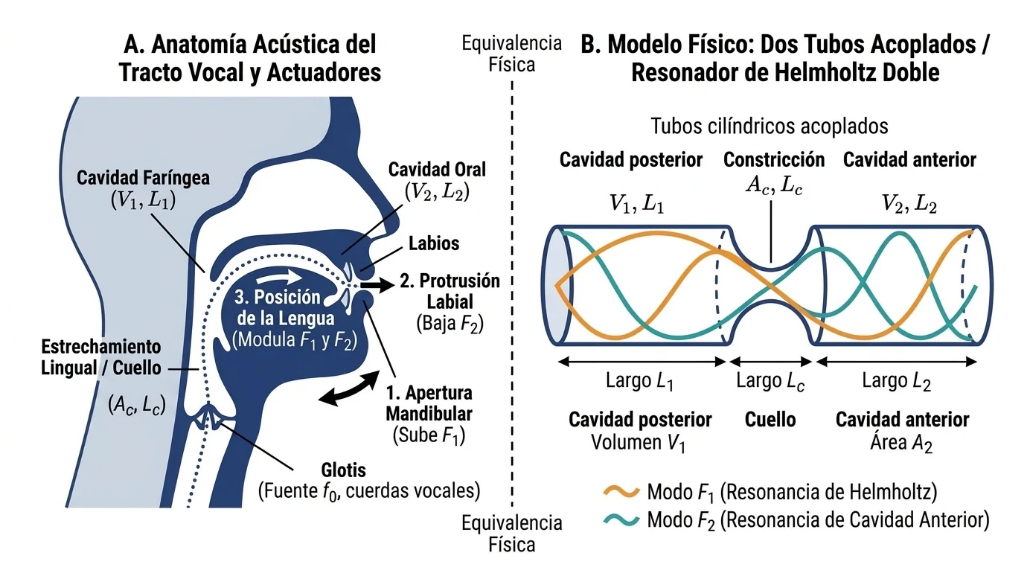
\includegraphics[width=\linewidth,height=0.72\textheight,keepaspectratio]{figuras/esquema_fisica_dos_tubos_helmholtz.png}
        \end{column}
    \end{columns}
\end{frame}

% ------------------------------------------------------------------------------
% Slide 2: El Mapa Acústico: Tres Puntos Cardinales y Vocales Intermedias
% ------------------------------------------------------------------------------
\begin{frame}{El Mapa Acústico: Tres Puntos Cardinales y Vocales Intermedias}
    \begin{columns}[c]
        \begin{column}{0.45\textwidth}
            \scriptsize
            \begin{block}{Topología en el Espacio de Formantes}
                Al proyectar las fonaciones en el plano espectral $F_1$ versus $(F_1 - F_2)$, la geometría articulatoria define un \textbf{triángulo vocal}:
                \begin{itemize}\setlength{\itemsep}{1pt}\setlength{\parskip}{0pt}
                    \item \textbf{Polos cardinales extremos:} Tres vértices fijos dados por \textbf{/a/}, \textbf{/i/} y \textbf{/u/}.
                    \item \textbf{Vocales intermedias:} Tanto la \textbf{/e/} como la \textbf{/o/} son estados físicos de transición a lo largo de las aristas del triángulo.
                \end{itemize}
            \end{block}
            \vspace{0.04cm}
            \begin{alertblock}{El Desafío Experimental de Sensado}
                \begin{itemize}\setlength{\itemsep}{1pt}\setlength{\parskip}{0pt}
                    \item Cada polo cardinal exige una configuración geométrica límite del tracto acústico.
                    \item \textbf{Pregunta de investigación:} ¿Cómo mapeamos de forma unívoca estos tres polos extremos utilizando únicamente tres canales de electromiografía de superficie?
                \end{itemize}
            \end{alertblock}
        \end{column}
        \begin{column}{0.53\textwidth}
            \centering
            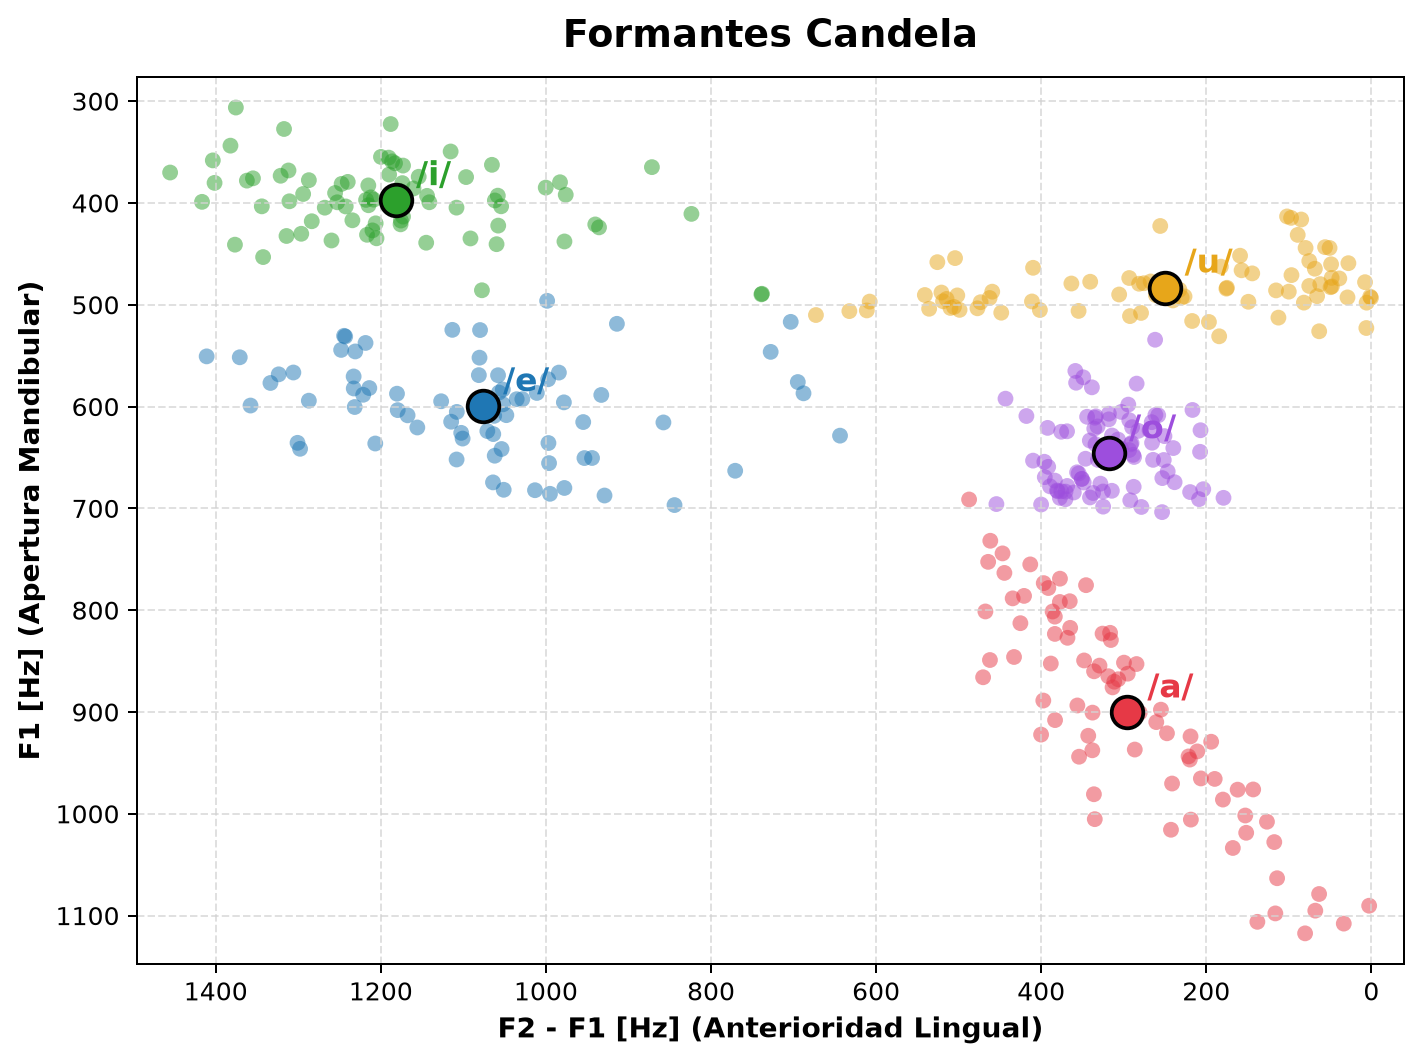
\includegraphics[width=\linewidth,height=0.37\textheight,keepaspectratio]{figuras/formantes_candela.png}\\[4pt]
            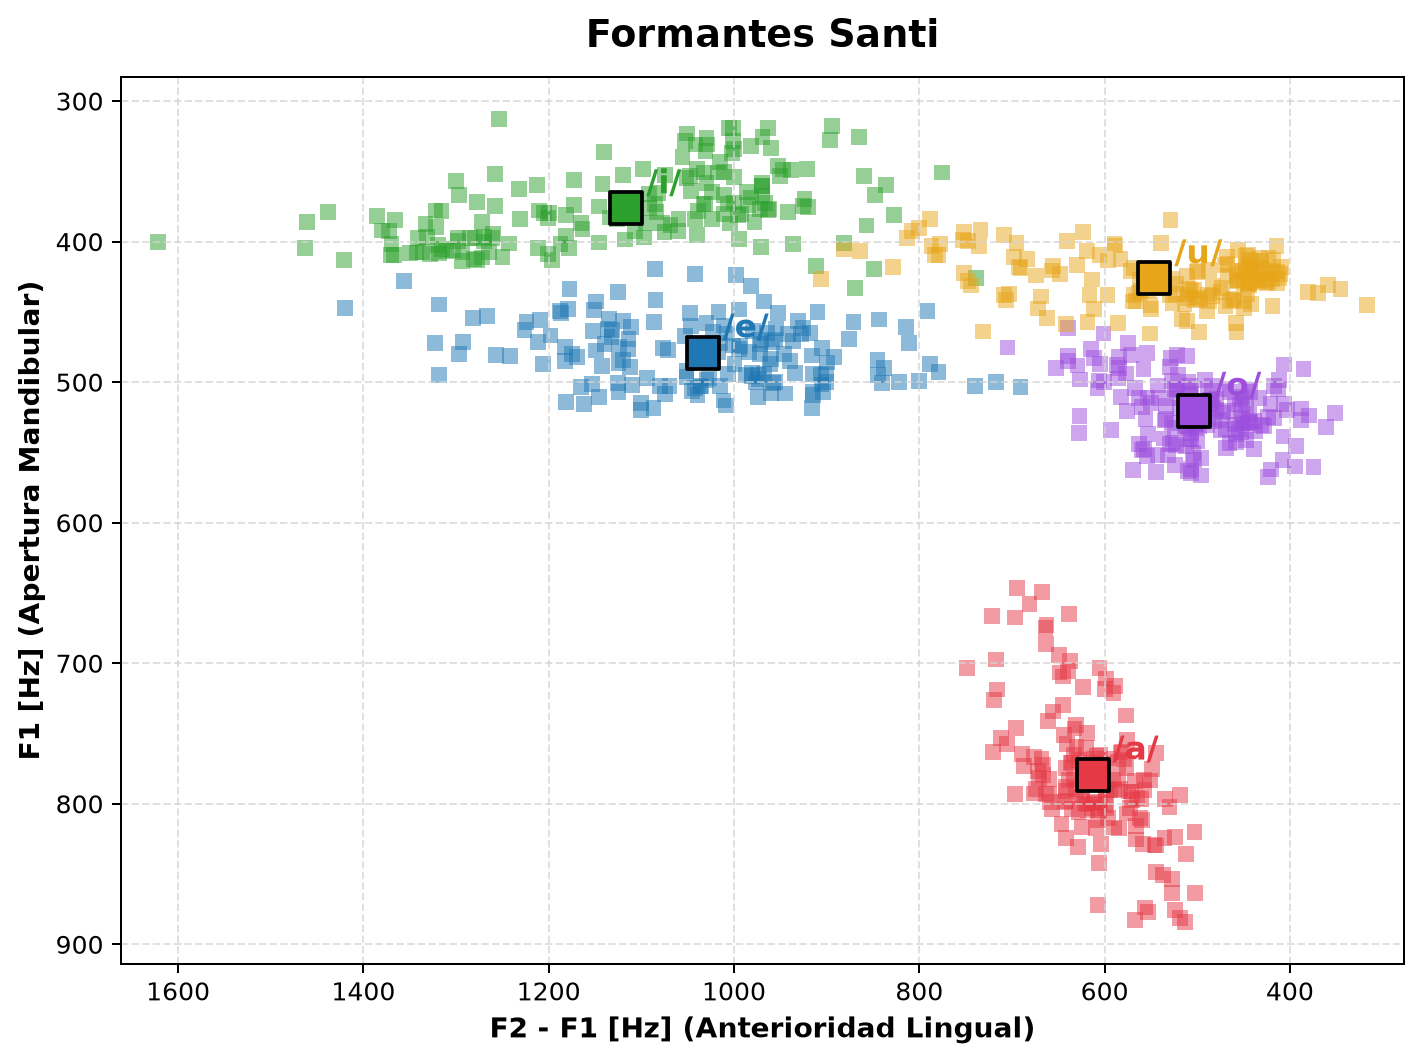
\includegraphics[width=\linewidth,height=0.37\textheight,keepaspectratio]{figuras/formantes_santi.png}
        \end{column}
    \end{columns}
\end{frame}

% ------------------------------------------------------------------------------
% Slide 3: Evidencia en Nuestras Mediciones: Los Polos que Funcionan Sólido - U y A
% ------------------------------------------------------------------------------
\begin{frame}{Evidencia en Nuestras Mediciones: Los Polos que Funcionan Sólido - U y A}
    \begin{columns}[c]
        \begin{column}{0.51\textwidth}
            \scriptsize
            \begin{block}{Polo Labial - Vocal /u/ y /o/}
                \begin{itemize}\setlength{\itemsep}{1pt}\setlength{\parskip}{0pt}
                    \item El músculo de los labios (\textit{orbicularis}) hace trompita hacia adelante y alarga el tubo resonador.
                    \item Causa física directa: señal limpia, ruido bajo y respuesta predecible en todos los sujetos.
                \end{itemize}
            \end{block}
            \vspace{0.03cm}
            \begin{block}{Polo de Apertura Mandibular - Vocal /a/}
                \begin{itemize}\setlength{\itemsep}{1pt}\setlength{\parskip}{0pt}
                    \item Para subir $F_1$ necesitamos abrir la boca bajando la mandíbula.
                    \item Registro sólido: activación clara debajo del mentón (\textit{digástrico}) y firmeza en la mandíbula (\textit{masetero}).
                \end{itemize}
            \end{block}
            \vspace{0.03cm}
            \begin{alertblock}{El Desafío Pendiente}
                Con dos polos resueltos físicamente, queda resolver con la misma certeza el tercer vértice: \textbf{la vocal /i/}.
            \end{alertblock}
        \end{column}
        \begin{column}{0.47\textwidth}
            \centering
            \placeholderfigura{0.72\textheight}{Señales / Envolventes representativas mostrando la activación limpia de Orbicularis en U y Digástrico en A}
        \end{column}
    \end{columns}
\end{frame}

% ------------------------------------------------------------------------------
% Slide 4: El Dilema de la Vocal I: Sonrisa - Correlación vs Lengua - Causa
% ------------------------------------------------------------------------------
\begin{frame}{El Dilema de la Vocal I: Sonrisa - Correlación vs Lengua - Causa}
    \begin{columns}[c]
        \begin{column}{0.51\textwidth}
            \scriptsize
            \begin{alertblock}{La Sonrisa en Mejilla no es la Causa Acústica}
                \begin{itemize}\setlength{\itemsep}{1pt}\setlength{\parskip}{0pt}
                    \item Al decir la /i/ se suele sonreír (\textit{cigomático}), pero es un gesto que solo acompaña.
                    \item La causa física real que sube $F_2$ es \textbf{empujar la lengua hacia adelante y arriba}.
                    \item Se puede pronunciar una /i/ limpia sin mover los labios, usando solo la lengua.
                \end{itemize}
            \end{alertblock}
            \vspace{0.1cm}
            \begin{exampleblock}{Qué Pasó en las Mediciones a lo Largo del Tiempo}
                Con los 3 sensores clásicos (\textit{Cigomático, Digástrico, Orbicular}):
                \begin{itemize}\setlength{\itemsep}{1pt}\setlength{\parskip}{0pt}
                    \item \textbf{Al principio:} Alta separación porque la sonrisa estaba acoplada a la /i/.
                    \item \textbf{Meses después:} El hablante sonrió también en la /a/, o hizo la /i/ solo con la lengua sin mover la cara, perdiendo separación.
                \end{itemize}
            \end{exampleblock}
        \end{column}
        \begin{column}{0.47\textwidth}
            \centering
            \placeholderfigura{0.70\textheight}{Comparativa de PCA del Sujeto 1: Antes - alta separabilidad vs. Después - colapso entre A, E, I por desacople del gesto de sonrisa}
        \end{column}
    \end{columns}
\end{frame}

% ------------------------------------------------------------------------------
% Slide 5: Donde Vive la Diferencia Real: El Mapa de Trevisan y Mindlin
% ------------------------------------------------------------------------------
\begin{frame}{Donde Vive la Diferencia Real: El Mapa de Trevisan y Mindlin}
    \begin{columns}[c]
        \begin{column}{0.51\textwidth}
            \scriptsize
            \begin{block}{Variables Mecánicas Directas - Trevisan y Mindlin}
                En el laboratorio se midieron las 3 variables de movimiento usando imanes y sensores Hall:
                \begin{itemize}\setlength{\itemsep}{1pt}\setlength{\parskip}{0pt}
                    \item \textbf{Labios:} Apertura y trompita hacia adelante (3 sensores).
                    \item \textbf{Mandíbula:} Bajar y subir la pera (apertura vertical).
                    \item \textbf{Lengua:} Posición hacia adelante, atrás o arriba.
                \end{itemize}
            \end{block}
            \vspace{0.04cm}
            \begin{alertblock}{La Coordenada Exclusiva de la Lengua}
                El gráfico de 3 dimensiones muestra un resultado contundente:
                \begin{itemize}\setlength{\itemsep}{1pt}\setlength{\parskip}{0pt}
                    \item \textbf{Para la /a/, /o/ y /u/:} La lengua casi no se mueve en ese eje; se separan solo con labios y mandíbula.
                    \item \textbf{Para la /i/ y la /e/:} La diferencia y separación de la /a/ ocurre \textbf{únicamente en el eje de la lengua}, donde la /i/ está en la posición máxima.
                \end{itemize}
            \end{alertblock}
        \end{column}
        \begin{column}{0.47\textwidth}
            \centering
            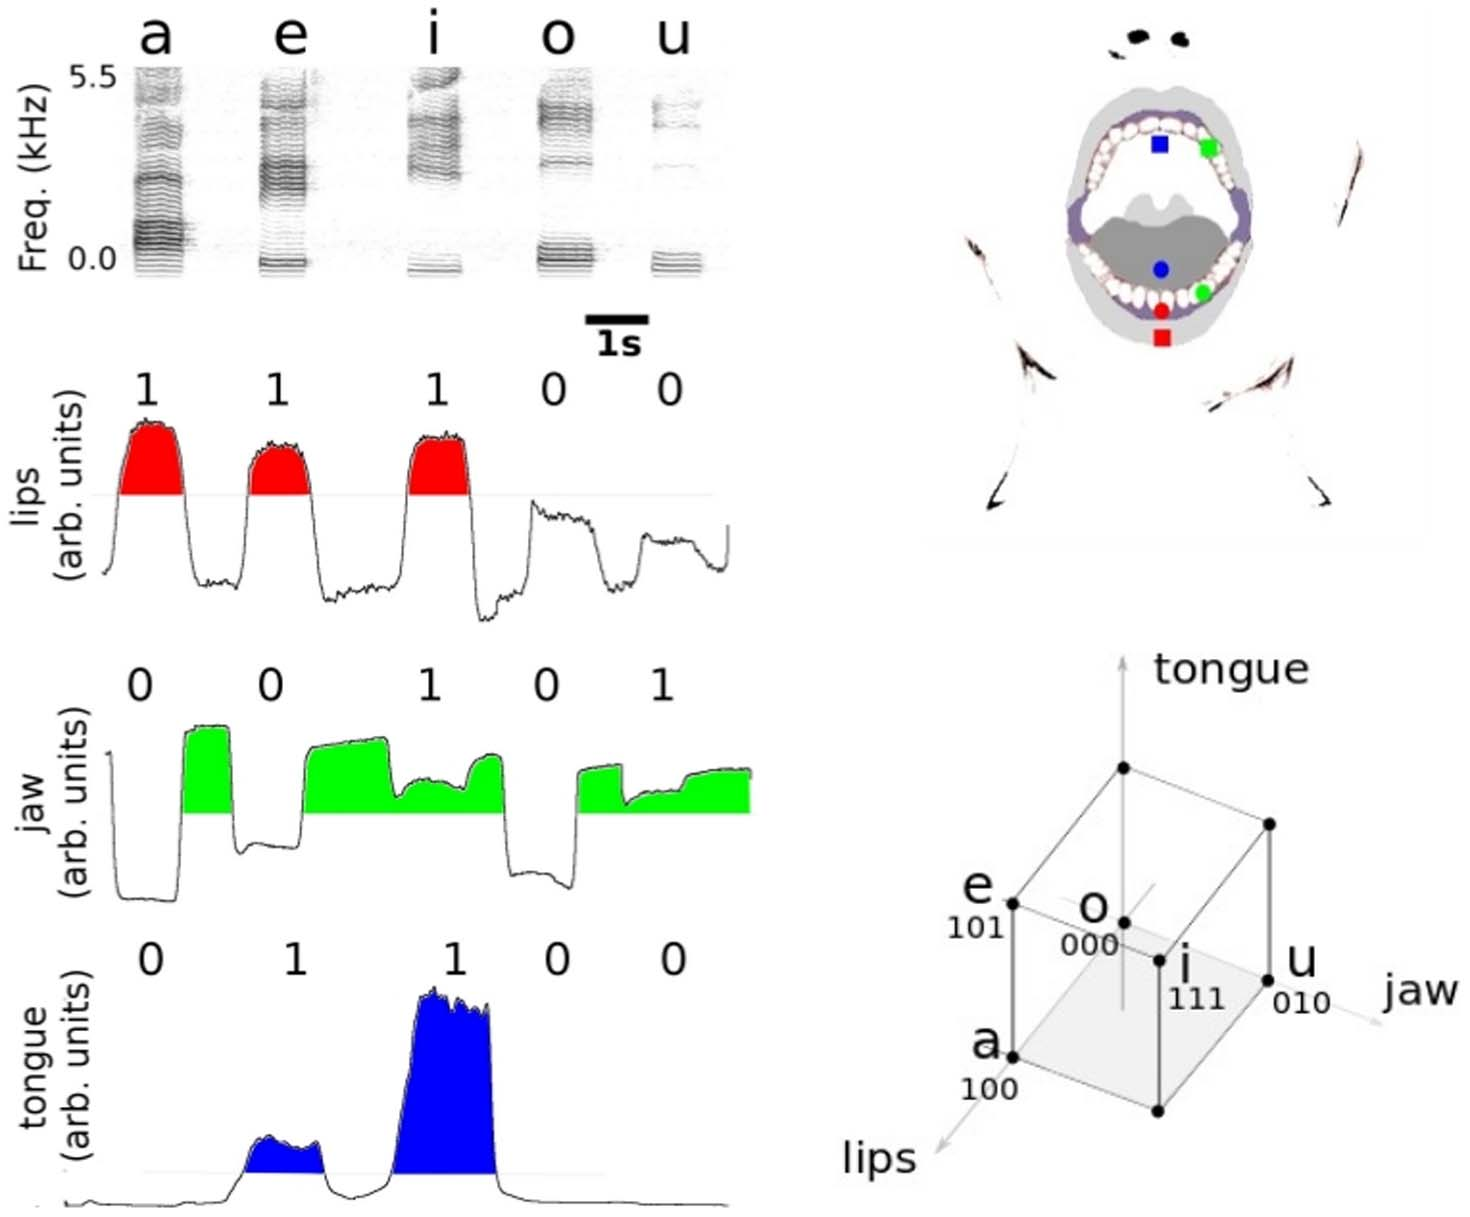
\includegraphics[width=\linewidth,height=0.72\textheight,keepaspectratio]{figuras/fig_trevisan_2013_cubo_articuladores.png}
        \end{column}
    \end{columns}
\end{frame}

% ------------------------------------------------------------------------------
% Slide 6: La Discusión de Fondo: Vocales Libres vs Gestos Entrenados
% ------------------------------------------------------------------------------
\begin{frame}{La Discusión de Fondo: Vocales Libres vs Gestos Entrenados}
    \begin{columns}[t]
        \begin{column}{0.48\textwidth}
            \scriptsize
            \begin{block}{Qué Miden los Sensores en la Cara}
                Los electrodos en la piel no leen el sonido, sino \textbf{los gestos que hace la cara al hablar}, que normalmente acompañan al sonido pero se pueden desacoplar.
            \end{block}
            \vspace{0.04cm}
            \begin{alertblock}{Hablar en Silencio - Sin Voz}
                Al fonoarticular sin emitir sonido:
                \begin{itemize}\setlength{\itemsep}{1pt}\setlength{\parskip}{0pt}
                    \item No hay aire saliendo ni sonido de referencia.
                    \item La persona tiende a relajar la cara o a mover la lengua adentro sin mover los labios.
                \end{itemize}
            \end{alertblock}
        \end{column}
        \begin{column}{0.48\textwidth}
            \scriptsize
            \begin{exampleblock}{Camino 1: Entrenar el Gesto Facial}
                \begin{itemize}\setlength{\itemsep}{1pt}\setlength{\parskip}{0pt}
                    \item Enseñar al usuario a marcar un gesto claro para cada vocal:
                    \begin{itemize}\setlength{\itemsep}{0pt}\setlength{\parskip}{0pt}
                        \item \textbf{/a/:} Abrir bien la boca hacia abajo.
                        \item \textbf{/i/:} Sonreír estirando hacia los costados.
                        \item \textbf{/u/:} Hacer trompita hacia adelante.
                    \end{itemize}
                    \item Funciona rápido y da clases limpias en poco tiempo.
                \end{itemize}
            \end{exampleblock}
            \vspace{0.04cm}
            \begin{block}{Camino 2: Medir la Lengua Directamente}
                \begin{itemize}\setlength{\itemsep}{1pt}\setlength{\parskip}{0pt}
                    \item Poner un sensor debajo de la mandíbula que lea la lengua.
                    \item Permite hablar con la cara relajada, pero hay que estudiar cómo cambia la fuerza al hablar en silencio.
                \end{itemize}
            \end{block}
        \end{column}
    \end{columns}
\end{frame}

% ------------------------------------------------------------------------------
% Slide 7: El Problema del Punto de Partida: Reposo, Vocales Intermedias y Coarticulación
% ------------------------------------------------------------------------------
\begin{frame}{El Problema del Punto de Partida: Reposo, Vocales Intermedias y Coarticulación}
    \begin{columns}[c]
        \begin{column}{0.51\textwidth}
            \scriptsize
            \begin{block}{Dinámica Muscular y Coarticulación}
                El electromiograma registra la fuerza para ir de una postura a otra: $\Delta \vec{x}(t) = \vec{x}_{\text{final}} - \vec{x}_{\text{inicial}}$.
                \begin{itemize}\setlength{\itemsep}{1pt}\setlength{\parskip}{0pt}
                    \item Si el hablante no afloja la cara entre letras, la posición de partida cambia continuamente.
                    \item \textbf{Paso de /e/ a /i/:} El movimiento restante es muy chico frente al trayecto desde el reposo.
                    \item \textbf{Efecto en el modelo:} Una /i/ que parte desde la /e/ produce la misma señal que una /e/ desde el reposo.
                \end{itemize}
            \end{block}
            \vspace{0.1cm}
            \begin{exampleblock}{Estandarizar la Tarea en el Laboratorio}
                Definir una regla fija para los ensayos: exigir volver a relajar la cara antes de cada vocal, o alimentar al modelo con la historia de la vocal previa.
            \end{exampleblock}
        \end{column}
        \begin{column}{0.47\textwidth}
            \centering
            \placeholderfigura{0.70\textheight}{Esquema o traza temporal mostrando la diferencia de amplitud al ir de Reposo -> I vs. ir de E -> I sin volver al reposo}
        \end{column}
    \end{columns}
\end{frame}

% ------------------------------------------------------------------------------
% Slide 8: Límites de los Sensores Actuales y Candidato para la Lengua
% ------------------------------------------------------------------------------
\begin{frame}{Límites de los Sensores Actuales y Candidato para la Lengua}
    \begin{columns}[c]
        \begin{column}{0.51\textwidth}
            \scriptsize
            \begin{alertblock}{Mezcla de Señales en las Posiciones Actuales}
                \begin{itemize}\setlength{\itemsep}{1pt}\setlength{\parskip}{0pt}
                    \item \textbf{Centro del mentón (digástrico):} Se activa al abrir la boca en la /a/, pero también salta si la lengua sube en la /i/, pisándose dos picos en el mismo canal.
                    \item \textbf{Mejilla (cigomático):} Activo al sonreír en la /i/, pero también se dispara en la /a/ si el hablante abre grande la boca hacia abajo.
                \end{itemize}
            \end{alertblock}
            \vspace{0.1cm}
            \begin{exampleblock}{Nueva Posición: Abajo del Mentón al Costado}
                Colocar un sensor en la \textbf{zona lateral debajo de la mandíbula} (lee la lengua sin el choque central) $+$ sensor de apertura $+$ sensor en labios (\textit{orbicular}). Cubre directamente las 3 variables del modelo de Trevisan y Mindlin.
            \end{exampleblock}
        \end{column}
        \begin{column}{0.47\textwidth}
            \centering
            \placeholderfigura{0.70\textheight}{Fotos / Mapa de ubicación de los electrodos mostrando la competencia de picos y la nueva posición submandibular lateral}
        \end{column}
    \end{columns}
\end{frame}

% ------------------------------------------------------------------------------
% Slide 9: Por Qué se Perdió la Separación: Ritmo, Pantalla y Cámara
% ------------------------------------------------------------------------------
\begin{frame}{Por Qué se Perdió la Separación: Ritmo, Pantalla y Cámara}
    \begin{columns}[c]
        \begin{column}{0.51\textwidth}
            \scriptsize
            \begin{block}{Hipótesis que Probamos Estas Semanas}
                \begin{itemize}\setlength{\itemsep}{1pt}\setlength{\parskip}{0pt}
                    \item \textbf{Anticiparse al metrónomo:} Quisimos evitar que la persona entre en automático agregando un atraso variable ($\Delta t$). Si el cambio de tiempo es muy rápido, se pierde todavía más el patrón (falta ajustar bien el rango de $\Delta t$).
                    \item \textbf{Mirar las ondas en la pantalla:} Ver la señal en vivo hacía que el usuario cambie la fuerza o corrija sobre la marcha. En los nuevos ensayos se usa \textbf{pantalla limpia} mostrando solo la letra a pronunciar.
                \end{itemize}
            \end{block}
            \vspace{0.03cm}
            \begin{alertblock}{La Cámara como Control del Experimento}
                \begin{itemize}\setlength{\itemsep}{1pt}\setlength{\parskip}{0pt}
                    \item \textbf{Uso exclusivo de control:} La cámara de video se usa únicamente para verificar el movimiento de la cara, nunca como parte del decodificador final (que es 100\% EMG).
                    \item \textbf{Prueba clave:} Si los puntos de la cara en la cámara tampoco separan las vocales en un PCA, confirmamos que la diferencia no está en el rostro sino adentro, en la lengua.
                \end{itemize}
            \end{alertblock}
        \end{column}
        \begin{column}{0.47\textwidth}
            \centering
            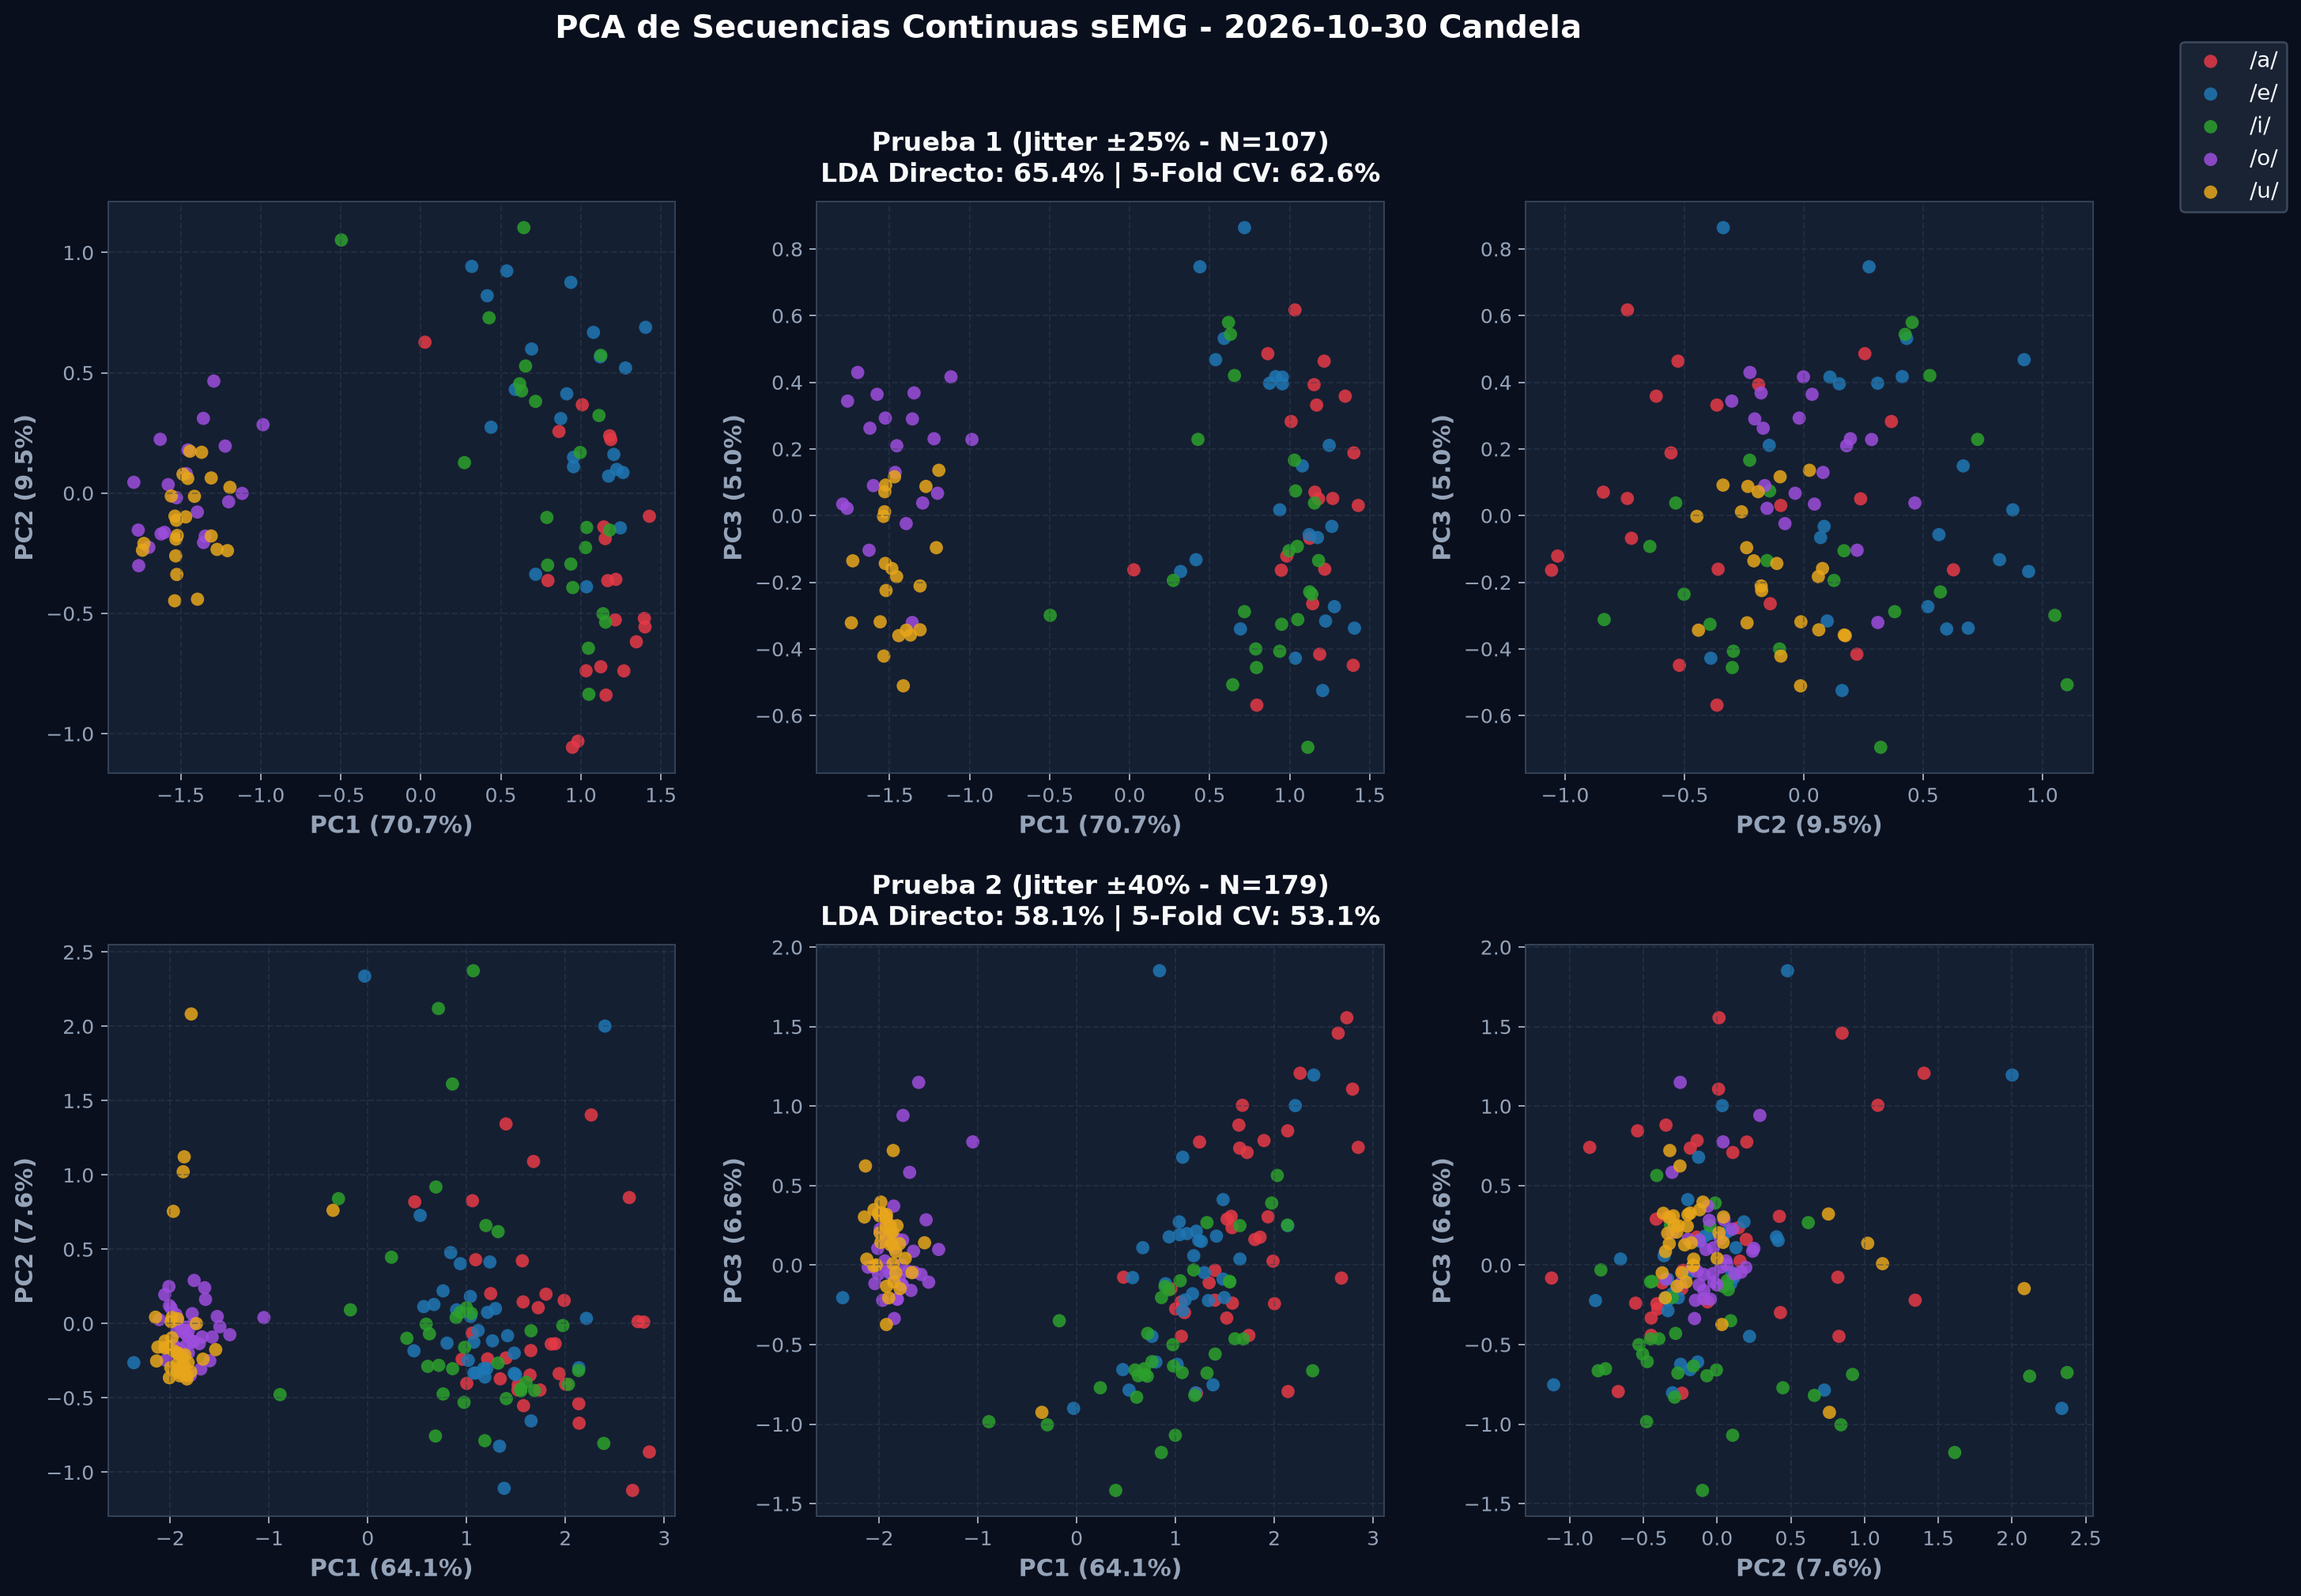
\includegraphics[width=\linewidth,height=0.72\textheight,keepaspectratio]{figuras/pca_comparativo_secuencias_continuas_jittering.png}
        \end{column}
    \end{columns}
\end{frame}

% ------------------------------------------------------------------------------
% Slide 10: Diseño de los Próximos Experimentos y las Tres Preguntas para la Mesa
% ------------------------------------------------------------------------------
\begin{frame}{Próximos Experimentos y Tres Preguntas para la Mesa}
    \begin{columns}[c]
        \begin{column}{0.48\textwidth}
            \scriptsize
            \begin{block}{Protocolos de Ritmo y Modos de Ejecución}
                \begin{itemize}\setlength{\itemsep}{0pt}\setlength{\parskip}{0pt}
                    \item \textbf{Ritmo en pantalla limpia:} Por bloques (\texttt{A-A-A...}), continuo parejo, o continuo con desfasaje ($\Delta t$) anti-anticipación.
                    \item \textbf{Modo Natural:} Pronunciación cotidiana libre del hablante.
                    \item \textbf{Modo Gesto Coordinado:} Reglas fijas (/a/: abrir boca, /e/: abrir $+$ sonreír, /i/: sonreír, /o/: abrir $+$ trompita, /u/: trompita sola).
                \end{itemize}
            \end{block}
            \begin{alertblock}{Tres Preguntas Clave para el Laboratorio}
                \begin{enumerate}\setlength{\itemsep}{0pt}\setlength{\parskip}{0pt}
                    \item ¿Buscamos clasificar \textbf{gestos coordinados} o \textbf{habla natural}?
                    \item ¿Podemos \textbf{re-acoplar el gesto} quitando la pantalla con señales y controlando el reposo?
                    \item ¿Sumamos el \textbf{sensor de lengua al costado bajo el mentón} para cubrir las 3 coordenadas de Trevisan?
                \end{enumerate}
            \end{alertblock}
        \end{column}
        \begin{column}{0.50\textwidth}
            \centering
            {\scriptsize \textbf{Modo Natural: Colapso A-E-I y O-U}}\\[1pt]
            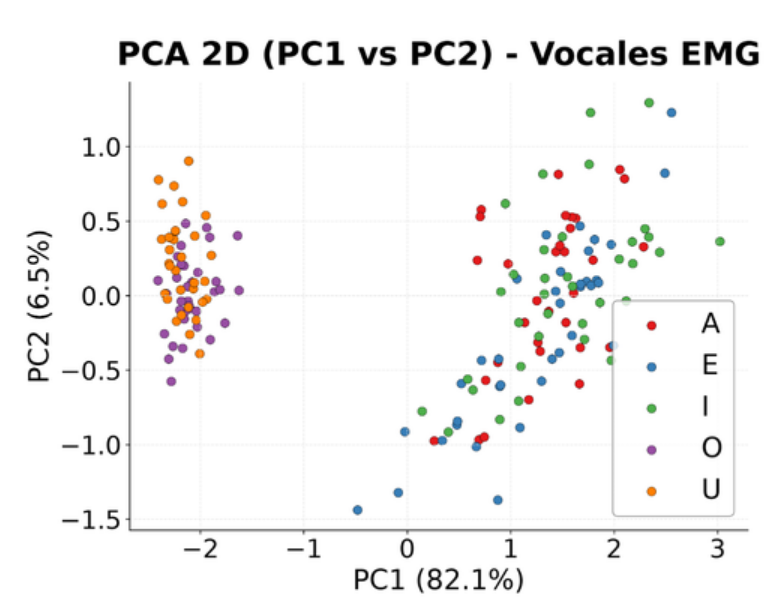
\includegraphics[width=\linewidth,height=0.29\textheight,keepaspectratio]{figuras/pca_vocales_modo_natural.png}\\[2pt]
            {\scriptsize \textbf{Modo Gesto Forzado: Separación Neta de I}}\\[1pt]
            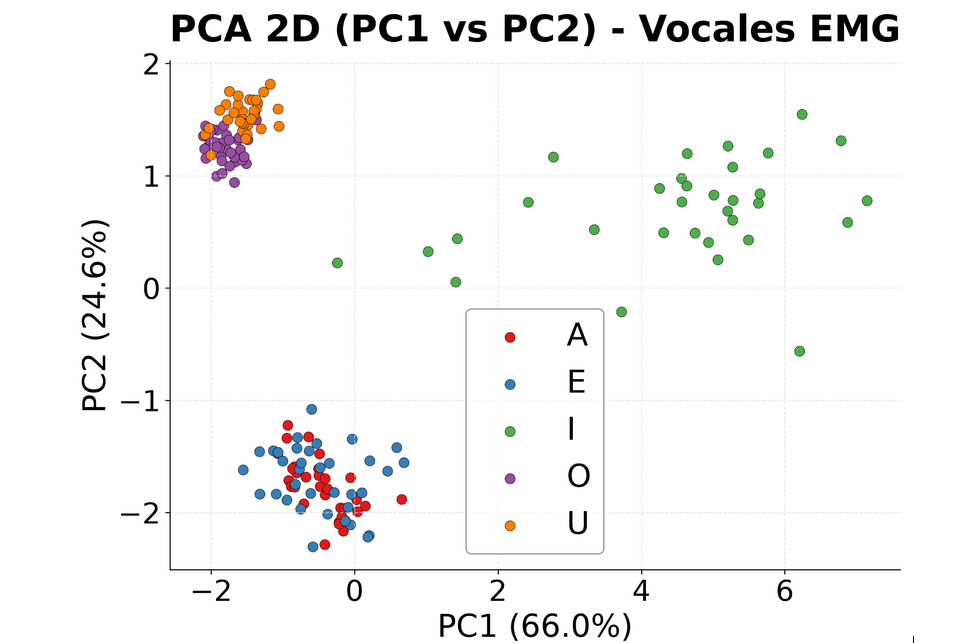
\includegraphics[width=\linewidth,height=0.29\textheight,keepaspectratio]{figuras/pca_vocales_modo_forzado.png}
        \end{column}
    \end{columns}
\end{frame}


\end{document}
